\section{Design of C-=-1}
\label{language-design}
C-=-1 is a new programming language, designed as low-level and non-garbage-collected and compiled to native machine code, similar to C, C++ or Rust.
What differentiates C-=-1 are its two core principles: all code is executable at compile-time and support for metaprogramming.
The primary purpose of this language was to investigate how these ideas influence software written in it \cite{grabski2022compilation}.

C-=-1 is a simple language, built with minimum set of features needed to demonstrate the usefulness of the proposed metaprogramming features.
They are discussed further in section  \ref{design:attributes_and_metaprogramming}.
The primary motivation for those mechanisms was to provide to a programmer the ability to create domain specific static analysis and code generation tools, without creating a separate program.

\subsection{Type system}

C-=-1 type system is similar to type system in C++.
Program may contain user defined classes, with members which may have limited accessibility. Generic programming is achieved by  templates, although they are much more limited than the ones present in C++.
The user may also use pointers to objects, with arbitrary indirection (for example pointer to pointer to object).
Additionally, the language contains the concept of an \lstinline{interface}, similar to the one found in C\#  \cite{hejlsberg2003c}.

\subsection{Attributes and metaprogramming}
\label{design:attributes_and_metaprogramming}

Metaprogramming in C-=-1 is based on attributes. Attributes work in a manner similar to the ones found in C\#.
They are types, which may contain fields and methods.
They can also be used to annotate other elements of the program, such as types, functions or variables.

In C-=-1 these attributes may implement special member functions that react to the use of an annotated program element.
For example, an attribute that can be attached to a function, may implement \lstinline{onCall} special member function.
It will be called at compile time, for each invocation of the annotated procedure.
Within the special method the attribute will have access to the semantic model of the call site.
It may then modify the semantic model or report warnings or errors.

Listing \ref{lst:noDiscardCm1} contains an example of a C-=-1 attribute providing static analysis: \lstinline{noDiscard}.
It works in the same manner as the attribute of the same name present in C++17 \cite{ISO:cpp17}: the result of invoking the annotated function must be used.
To declare an attribute in C-=-1, the \lstinline{att} keyword is used.
After that, attribute targets should be listed in angled brackets, as in line 0 of Listing \ref{lst:noDiscardCm1}.
Valid targets for attributes include a number of language elements, such as types, functions, variables and fields. Attribute from Listing \ref{lst:noDiscardCm1} declares two member functions: \lstinline{attach} in line 4 and \lstinline{onCall} in line 6.
Listing \ref{lst:noDiscardUsageCm1} contains an example of using the \lstinline{noDiscard} attribute.
All uses of the \lstinline|noDiscardFunction|, except for the one on line 3 are valid.
Using the function in a statement as opposed to an expression causes a compile-time error.

The \lstinline{attach} method is called after names of all program elements have been gathered, but before compiler starts to analyze function bodies.
It is common among all attribute targets and accepts the descriptor of the attached program element (function, field, type, etc.).
Attribute can change aspects of the program that affect function overload resolution, such as  whether a function is invokable at run or compile time, only from within the \lstinline{attach} method.

The \lstinline{onCall} method is an example of a function reacting to use an annotated program element.
These methods are specific to a given attribute target.
Within this function, the attribute may analyze and modify the code, as well as raise errors or warnings.

\begin{minipage}{\linewidth}

	\begin{lstlisting}[
	  numbers=left,
	  firstnumber=0,
	  caption={noDiscard attribute in C-=-1},
	  aboveskip=0pt,
	  label={lst:noDiscardCm1}
	  ]
public att<function> NoDiscard
{
	public fn attach(f: functionDescriptor)
	{}
	public fn onCall(call: functionCallExpression*)
	{
		if(call._parentStatment != null<IInstruction>())
			raiseError(
			&(call._pointerToSource),
			"Return value of a no-discard function is not used",
			123
			);
}
}
  \end{lstlisting}
\end{minipage}



Lines 6 to 11 of Listing \ref{lst:noDiscardCm1} are an example of a C-=-1 attribute providing static analysis.
The \lstinline{onCall} method checks whether the attached function is invoked in an expression or instruction context.
Calling a function as a statement means that the result of that invocation is discarded by the caller.
This may indicate an error, when the function has no other side effects.
If that is the case, the attribute calls the \lstinline{raiseError} function, which is provided as a compiler intrinsic, that generates a compilation error.
The example presented in Listing \ref{lst:noDiscardCm1}, although very basic, demonstrates the ability to implement a form of static analysis that typically requires modifying the compiler or creating an external tool.

\begin{minipage}{\linewidth}

	\begin{lstlisting}[
	  numbers=left,
	  firstnumber=0,
	  caption={Example of using noDiscard attribute from Listing \ref{lst:noDiscardCm1}},
	  aboveskip=0pt,
	  label={lst:noDiscardUsageCm1}
	  ]
  [noDiscard()]
  fn noDiscardFunction() -> usize;
  fn main() -> usize {
	noDiscardFunction();
	// error 123: Return value of
	// a no-discard function is not used
	let x = noDiscardFunction();     // ok
	let y = x + noDiscardFunction(); // ok
	return noDiscardFunction();      // ok
  }
  \end{lstlisting}
\end{minipage}

\section{Design of the compiler}
\label{compiler-design}

CTFEF approach was created during implementation of the first compiler for the C-=-1 language\cite{grabski2022compilation}.
CTFEF compiler has four major components:
\begin{enumerate}
	\item Frontend.
	\item Interpreter.
	\item Compiler Interface.
	\item Backend.
\end{enumerate}

Figure \ref{CTFE-first-compiler-structure} contains a diagram with an overview of how these parts interact with each other, during the compilation process.
Frontend, described in section \ref{Frontend}, parses the code in the compiled language and constructs its intermediate representation, using Interpreter's data structures.
The structure and form of the intermediate representation is not specified by the CTFEF approach, as long as it contains all semantically relevant information from the source program.
It is used to analyze both user code and the Compiler Interface.
After the intermediate representation is constructed, it is passed to the Interpreter, which is described in section \ref{Interpreter}.
Compiler Interface intermediate representation is then executed, using the user program as data.
This step converts the semantic model of the program into the Backends intermediate language.
This process is further explained in section \ref{compiler-interface}.
Finally, the Backend generates the executable file.

\begin{figure}
	\centering
	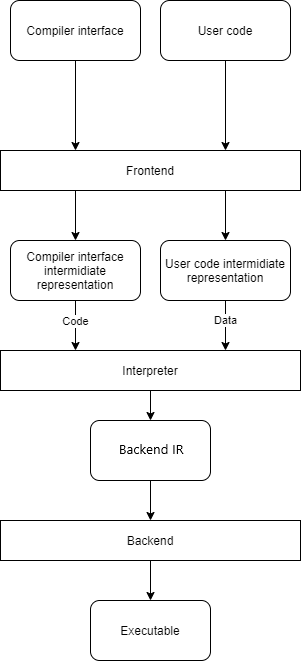
\includegraphics[height=13cm]{pictures/compiler-structure.png}
	\caption{CTFEF compiler structure}
	\label{CTFE-first-compiler-structure}
\end{figure}

\subsection{Frontend}
\label{Frontend}

In the CTFEF approach, Frontend serves the same role of constructing the programs intermediate representation, as in conventional compilers \cite{puntambekar:compiler_design}.
The major difference lays in the data structures used to describe the program.
For a CTFEF compiler, they must be accessible to the program running within the Interpreter.
This may make Frontend more complex.
The additional challenge of representing a user program, using Interpreter data structures, depends on the design of the Interpreter.


\subsection{Interpreter}
\label{Interpreter}

In CTFEF, Interpreter is main component of the compiler.
It executes the Compiler-Interface which translates the intermediate representation into the Backend's assembly and serves as what is sometimes called the 'middle-end' of the compiler\cite{hsu2021llvm}.
To do it, it must be able to treat the program's intermediate representation both as code and data.

\begin{figure}
	\centering
	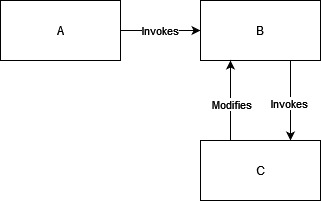
\includegraphics[width=7cm]{pictures/circular-function-reference.jpg}
	\caption{Example of circular reference in meta code}
	\label{circular-function-reference}
\end{figure}

An important issue for CTFEF compiler is decision what code can be executed at compile-time.
In some languages it may be possible to introduce circular references between the functions that modify the codebase.
Figure \ref{circular-function-reference} contains a diagram of such scenario.
\lstinline{A}, \lstinline{B} and \lstinline{C} are functions.
If function \lstinline{B} is modified by function \lstinline{C} and \lstinline{B} invokes \lstinline{C}, the behavior of function \lstinline{A} is unpredictable.
This problem will only be magnified by larger program sizes.

One of possible solutions, to the above-mentioned problem, is to restrict which functions can be invoked at compile time.
C-=-1 allows code within a compile time context to invoke procedures only from other packages, declared explicitly as dependencies.
Circular references between packages, as in most other languages, are forbidden.
C-=-1 additionally  prohibits modification of dependencies.
Therefore, it is impossible for a function to modify a procedure, it depends on.

\subsection{Compiler Interface}
\label{compiler-interface}

Compiler Interface translates the program's intermediate representation into the Backend's assembly language.
This component is interpreted during compilation and may be provided by the user.
In case of C-=-1, compiler interface could be supplied to the compiler, the same way that the code being compiled is passed, as a collection of source files.
Figure \ref{compiler-design} reflects this decision, treating the Compiler Interface as an input into the compiler, same as user code.

What is unique about CTFEF is that this part of the compiler can be written in the target language, during initial bootstrapping of the compiler bootstrapping process, i.e. initial implementation using another language \cite{puntambekar:compiler_design, novillo2007gcc}.
In case of the C-=-1 compiler, C++ was used to implement Frontend, Backend and Interpreter, with Compiler Interface written in C-=-1 \cite{grabski2022compilation}.

Compiler Interface contains a function marked as the Compiler Interface Entry-point.
That procedure must accept a set of modules to be compiled and a Compilation Context that is used to generate the Backends assembly.
The module descriptors that are passed to the Compiler Interface are built by the Frontend, as can be seen in Figure \ref{CTFE-first-compiler-structure}.

After the Compiler Interface finishes generating Backend assembly, the Compiler Backend is invoked to generate the binary executable.
\subsection{Backend}
\label{Backend}

CTFEF does not put any additional requirements on compiler Backend.
When using this approach, a generic Backend library can be used.
C-=-1 compiler used LLVM\cite{lattner2008llvm} as its backend.

The Backend code must be invokable from within the interpreted program in the target language.
Depending on how the Interpreter was designed, this may require significant effort. %todo: maybe other word
Compiler Backends are large and for the Compiler Interface to take advantage of them, their entire interface must be fully available in the interpreted context.
This means exposing each function and type within the library to the interpreted code, by duplicating their signatures.
These bindings could feasibly be generated automatically \cite{marshalling_auto_generation}, but this technique was not used when implementing C-=-1 compiler.
